\documentclass{article}
\usepackage[spanish]{babel}
\usepackage[utf8]{inputenc}
\usepackage{graphicx}
\usepackage{amsmath}
\usepackage{amssymb}
\usepackage{amsthm}
\usepackage{wrapfig}

\begin{document}

\title{\textbf{Proyecto \#3 DAA:} La venganza de Alejandra}
\author{L\'azaro Daniel Gonz\'alez Mart\'inez y Alejandra Monz\'on Pe\~na}

\date{}
\maketitle

\section*{Desccripci\'on del problema}
Dado un grafo $G$, eliminar aristas hasta que todos sus v\'ertices sean de grado $3$ o $0$, sin eliminarlas todas.\\ 

Esto es equivalente a determinar si un grafo $G$ tiene un subgrafo $G^{'}$ regular de grado $3$. \\

Los grafos regulares de grado $3$ se conocen tambi\'en como \textit{grafos c\'ubicos}, por lo que usaremos ambos t\'erminos indistintamente.

\section*{Reducci\'on de 3-coloreable a subgrafo 3-regular}
Primero, demostrar que el problema de subgrafo c\'ubico (CSP [cubic subgraph problem]) cumple $ CSP \subseteq NP$ es sencillo, ya que si tuvi\'esemos un grafo $G$ y conoci\'eramos 
qué aristas de \'el componen el subgrafo c\'ubico, basta con recorrer el conjunto $E$ de aristas a conservar del grafo $G$ como parte del subgrafo c\'ubico 
y por cada par de v\'ertices sobre los que incide aumentar en $1$ su degree, finalmente basta con recorrer la lista de v\'ertices de $G$ y comprobar que todos tengan degree 
$0$ o  $3$(y al menos se tuviera una arista), procedimiento cuyo costo ser\'ia $O(|V| + |E|)$, como existe una forma polin\'omica de comprobar si una instancia del problema realmente cumple con 
la caracter\'istica deseada. Queda entonces demostrar que el problema $CSP = NP$.\\

Para demostrar que el problema de determinar si un grafo tiene un subgrafo c\'ubico es NP-completo, es necesario hacer una reducci\'on de un problema que sea NP-completo 
a este problema; para esto utilizaremos el problema $3$-coloreable, ya que el problema de la 3-coloraci\'on de un grafo se demostr\'o NP-completo por Karps.\\

Definamos t\'erminos a utilizar en la demostraci\'on: 
\begin{itemize}
    \item[$\ast $] $G$: grafo de entrada del problema 3-coloreable.
    \item[$\ast $] $V(G)~ = ~\{v_1,~ v_2,~ ... ~, ~v_n\}$: v\'ertices de $G$.
    \item[$\ast $] $E(G)~ = ~\{e_1, ~e_2,~ ...~ ,~ e_m\}$: aristas de $G$.
    \item[$\ast $] $<u,v>$: Arista que conecta los v\'ertices $u$ y $v$
    \item[$\ast $] $d(v_i)$: Grado del v\'ertice $v_i$.
    \item[$\ast $] $\Delta(G)$: Mayor degree de los v\'ertices del grafo.
    \item[$\ast $] $K^{'}_n$: Grafo completo de $n$ v\'ertices al que se le quita una arista(tiene todos los v\'ertices con degree n-1, excepto 2 v\'ertices de degree n-2).
    \item[$\ast $] $3$-partici\'on de $V(G)$: Conjuntos $V_1$, $V_2$ y $V_3$, tales que $\bigcup_{i=1}^{3} ~V_i~ = ~V(G)$  y $V_i ~\cap~ V_j~ =~ \emptyset$ para todo $i~ \neq~ j$.
\end{itemize}

\textbf{Transformaci\'on de la entrada:}\\

A partir del grafo $G$ se construye un nuevo grafo $G'$ de la siguiente forma:\\ 

\begin{wrapfigure}{R}{5cm}
    \centering
    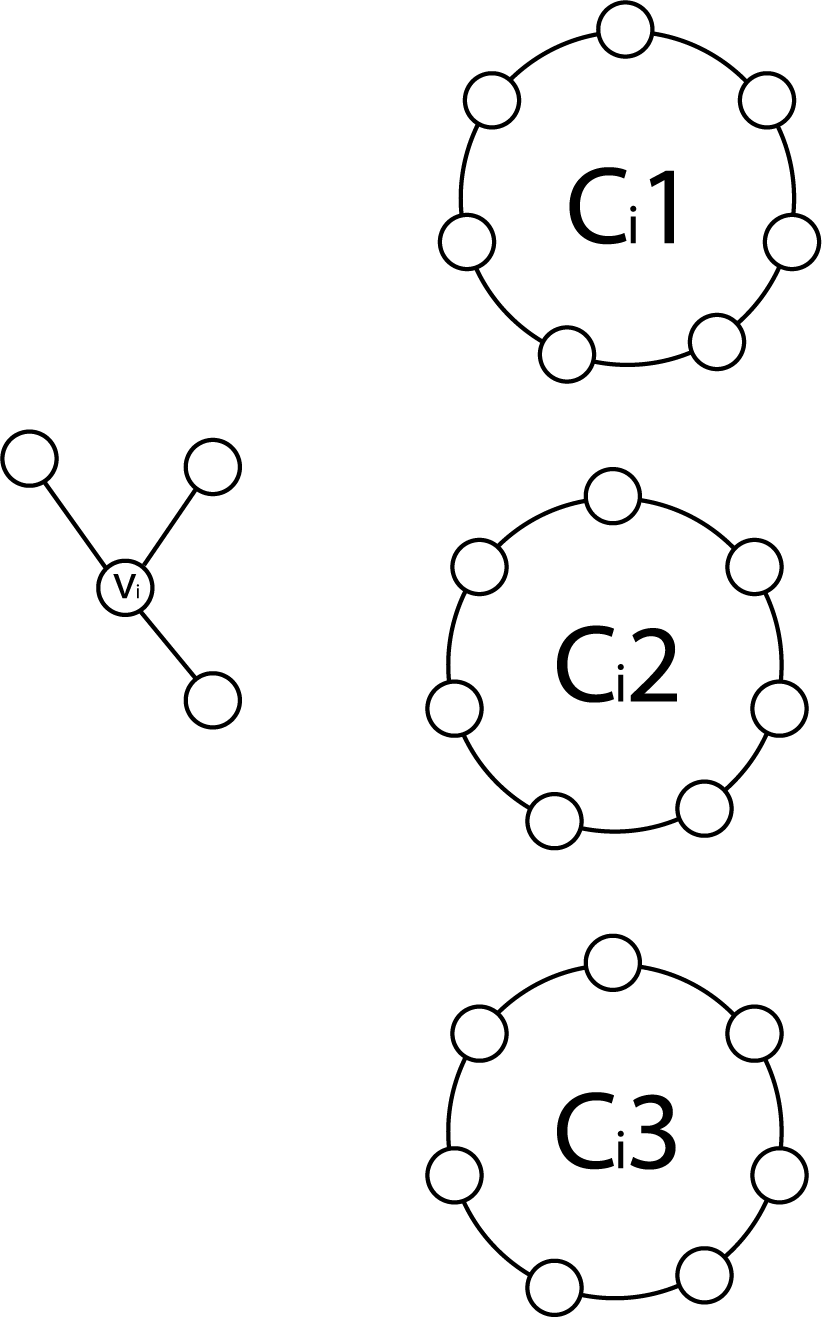
\includegraphics[width= 0.2\textwidth]{img1.png}
\end{wrapfigure}

1 - Por cada $v_i$ de $V(G)$ se crean $3$ ciclos $C_i^1$, $C_i^2$ y $C_i^3$, cada uno de longitud igual a $2 ~*~ d(v_i)~ + ~1$. Denotemos 
los v\'ertices de cada ciclo $C_i^h$ como $c_{ij}^h$, $1~ \leq~i~\leq ~n$, $1~ \leq~d~\leq ~2 ~*~ d(v_i)~ + ~1$, $1~ \leq~h~\leq ~3$.\\ 


2 - Por cada $e_j$ de $E(G)$ se crean $3$ subgrafos $D_{j}^1$, $D_{j}^2$ y $D_{j}^3$ en $G'$, donde cada $D_{j}^h$, $1~ \leq~h~\leq ~3$,  es un $K^{'}_4$, a los dos v\'ertices 
de $D_{j}^h$ con grado $2$ los denotaremos como $x_{j}^h$ y $y_{j}^h$.\\
\begin{wrapfigure}{L}{5cm}
    \centering
    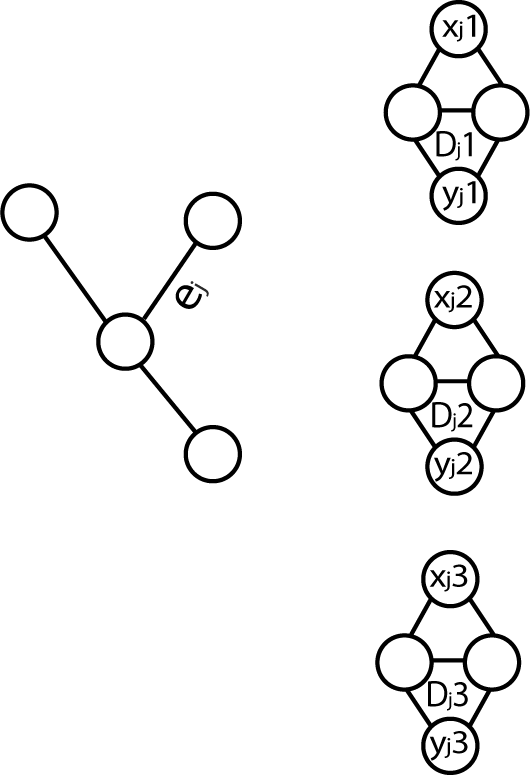
\includegraphics[width= 0.2\textwidth ]{img2.png}
\end{wrapfigure}


3 - Por cada $e_j$, sean $v_s$ y $v_t$ los v\'ertices sobre los que incide en $G$, de los ciclos $C_s^h$ ($C_t^h$) se toman $2$ v\'ertices 
$c_{s\alpha}^h$ y $c_{s\beta}^h$ ($c_{s\alpha}^h$ y $c_{s\beta}^h$) que aun tengan degree $2$; por cada $1~\leq ~h ~\leq~ 3$ se agregan a $G'$ las aristas: $<c_{s\alpha}^h, x_{j}^h>$, $<c_{s\beta}^h, y_{j}^h>$, 
$<c_{t\alpha}^h, x_{j}^h>$ y $<c_{t\beta}^h, y_{j}^h>$.\\ 

Una vez consideradas todas las aristas en el paso (3), se tiene que para cada ciclo $C_i^h$ ( $1~\leq ~i ~\leq~ n$, $1~\leq ~h ~\leq~ 3$ )
solo queda un v\'ertice con degree $2$. Nombremos dichos v\'ertices como $w_i^h$.\\ 
\begin{figure}[!h]
    \centering
    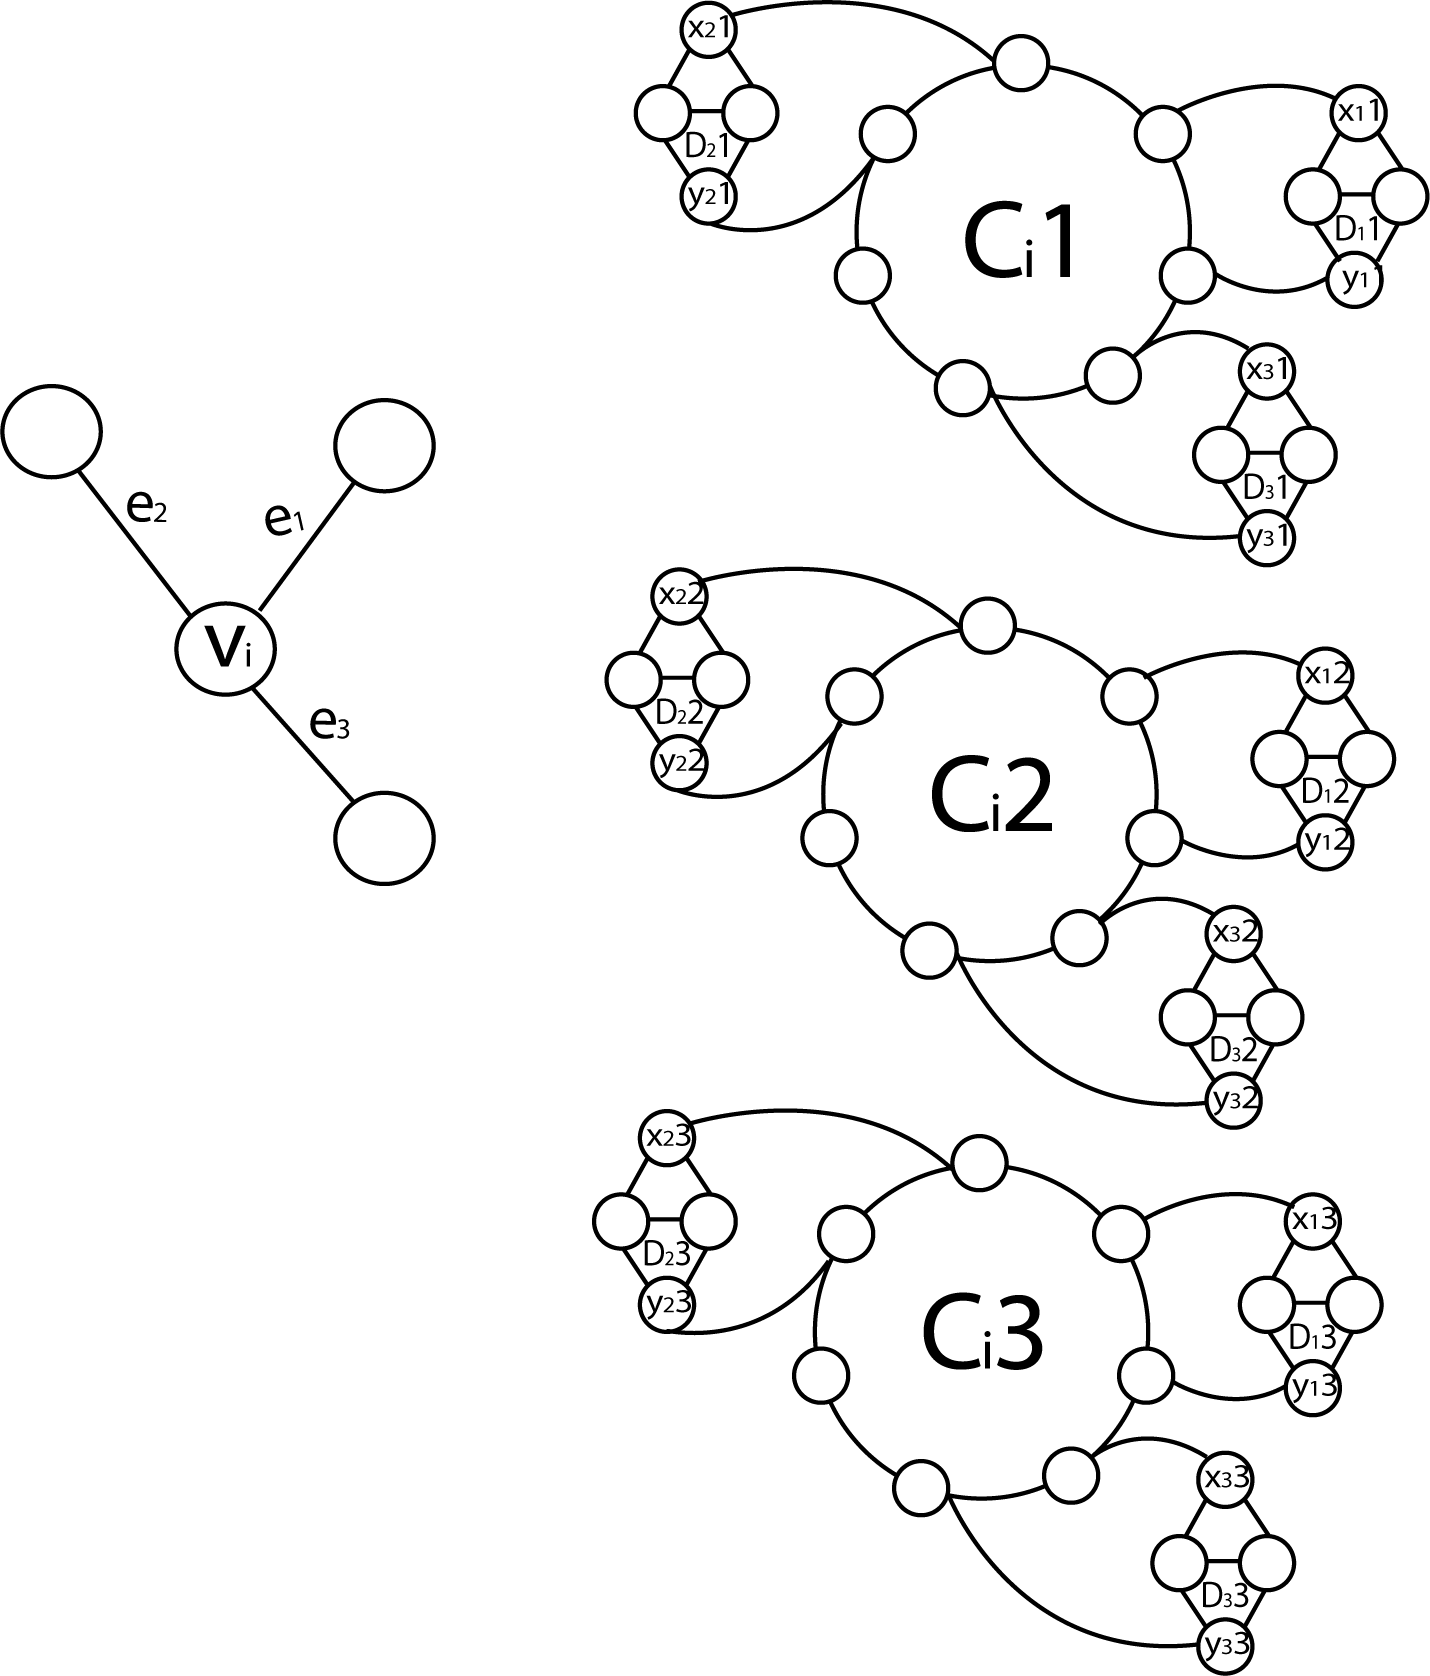
\includegraphics[width= 0.5\textwidth ]{img3.png}
\end{figure}

4 - Por cada $1~\leq ~i ~\leq~ n$, se construye un subgrafo $U_i$, que es un $K^{'}_4$ m\'as un v\'ertice al que denominaremos $u_{i}$, los v\'ertices de grado $2$ del $K^{'}_4$
los denominaremos $x_{i}$ y $y_{i}$, el v\'ertice $u_i$ se une a los restantes del  $K^{'}_4$ mediante una arista $<x_{i},u_i>$.\\ 



Se toman todos los grafos $U_i$ y se agregan a $G'$, junto con las aristas: $<u_i, w_i^1>$, $<y_i, w_i^2>$ y $<y_i, w_i^3>$. \\

\begin{figure}[!h]
    \centering
    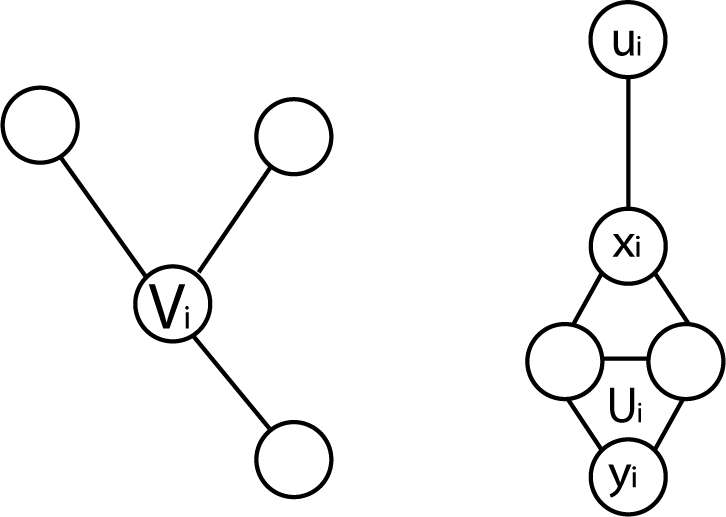
\includegraphics[width= 0.4\textwidth ]{img4.png}
    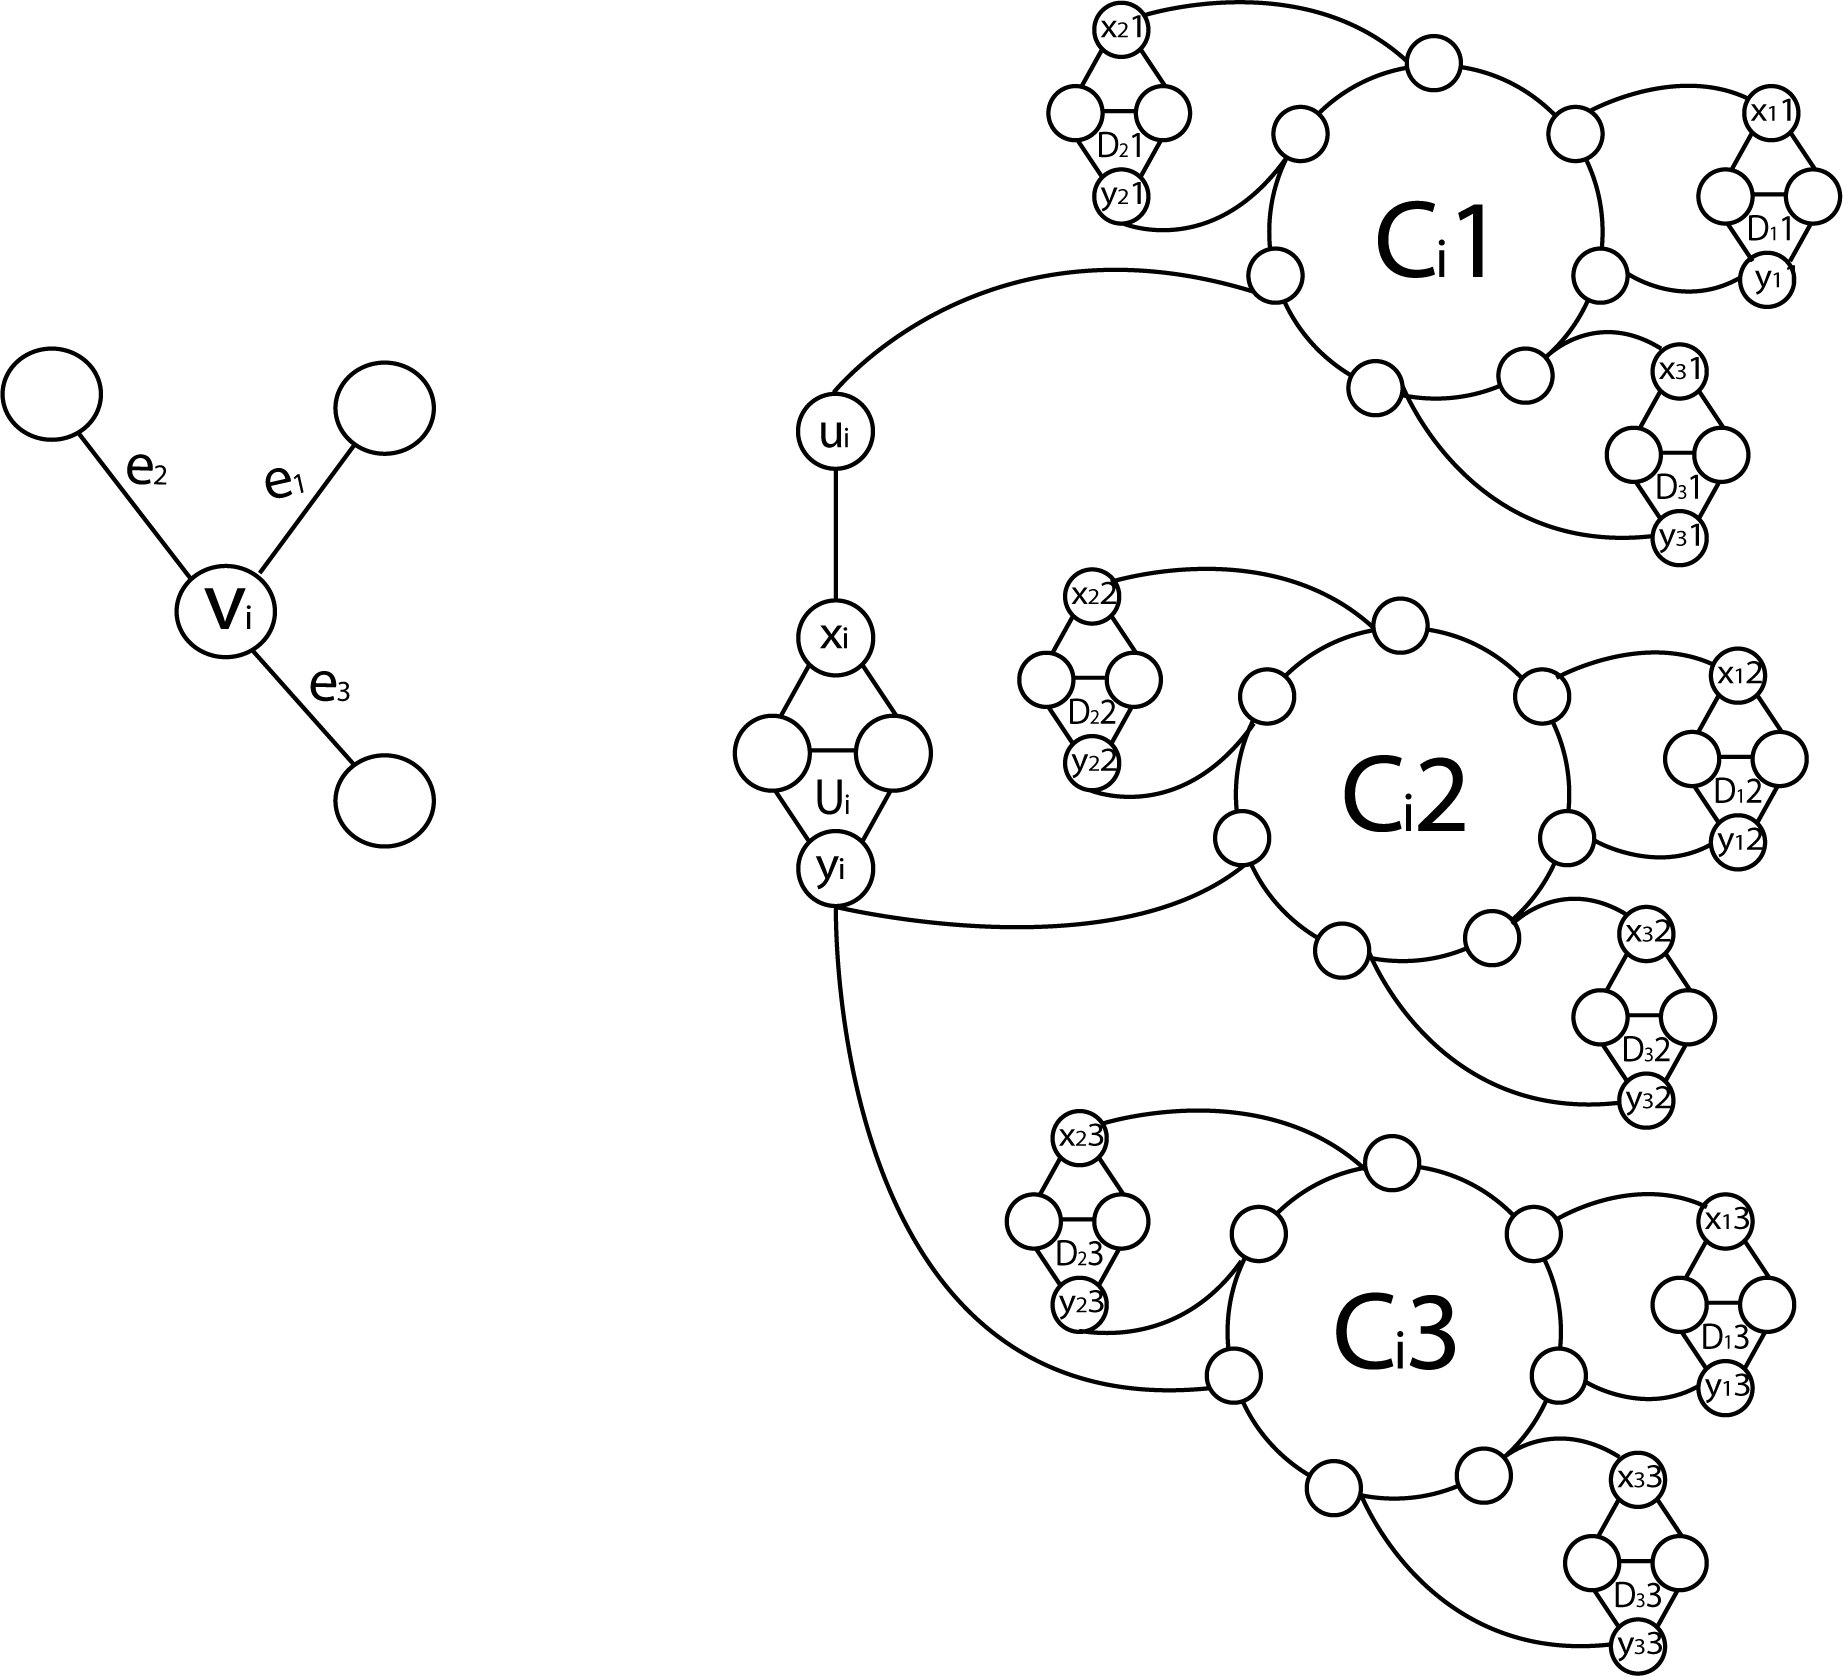
\includegraphics[width= 0.3\textwidth ]{img5.png}
\end{figure}

5 - Agregar el ciclo $C'$ de longitud $2~*~n$ a $G'$, conformado por los v\'ertices: $\{ a_{11}, ... , a_{1n}, a_{21}, ... , a_{2n} \}$ y agregar las aristas 
$<a_{pi}, u_{i}>$ para $p = 1,2$.\\
\begin{figure}[!h]
    \centering
    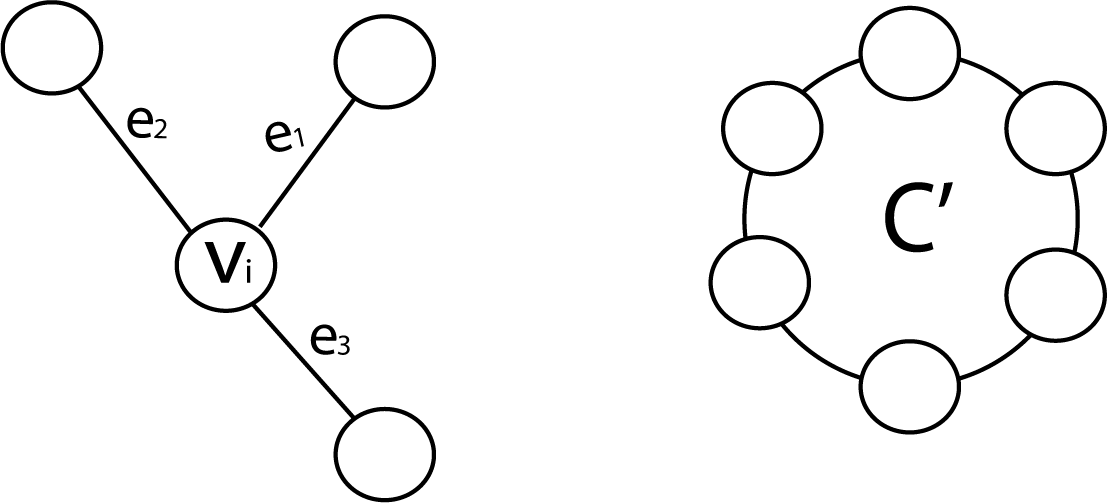
\includegraphics[width= 0.3\textwidth ]{img6.png}
\end{figure}

Construido $G'$, queda demostrar que en $G$ es $3$-coloreable si y solo si $G'$ tiene un subgrafo c\'ubico. \\ 

\begin{figure}[!h]
    \centering
    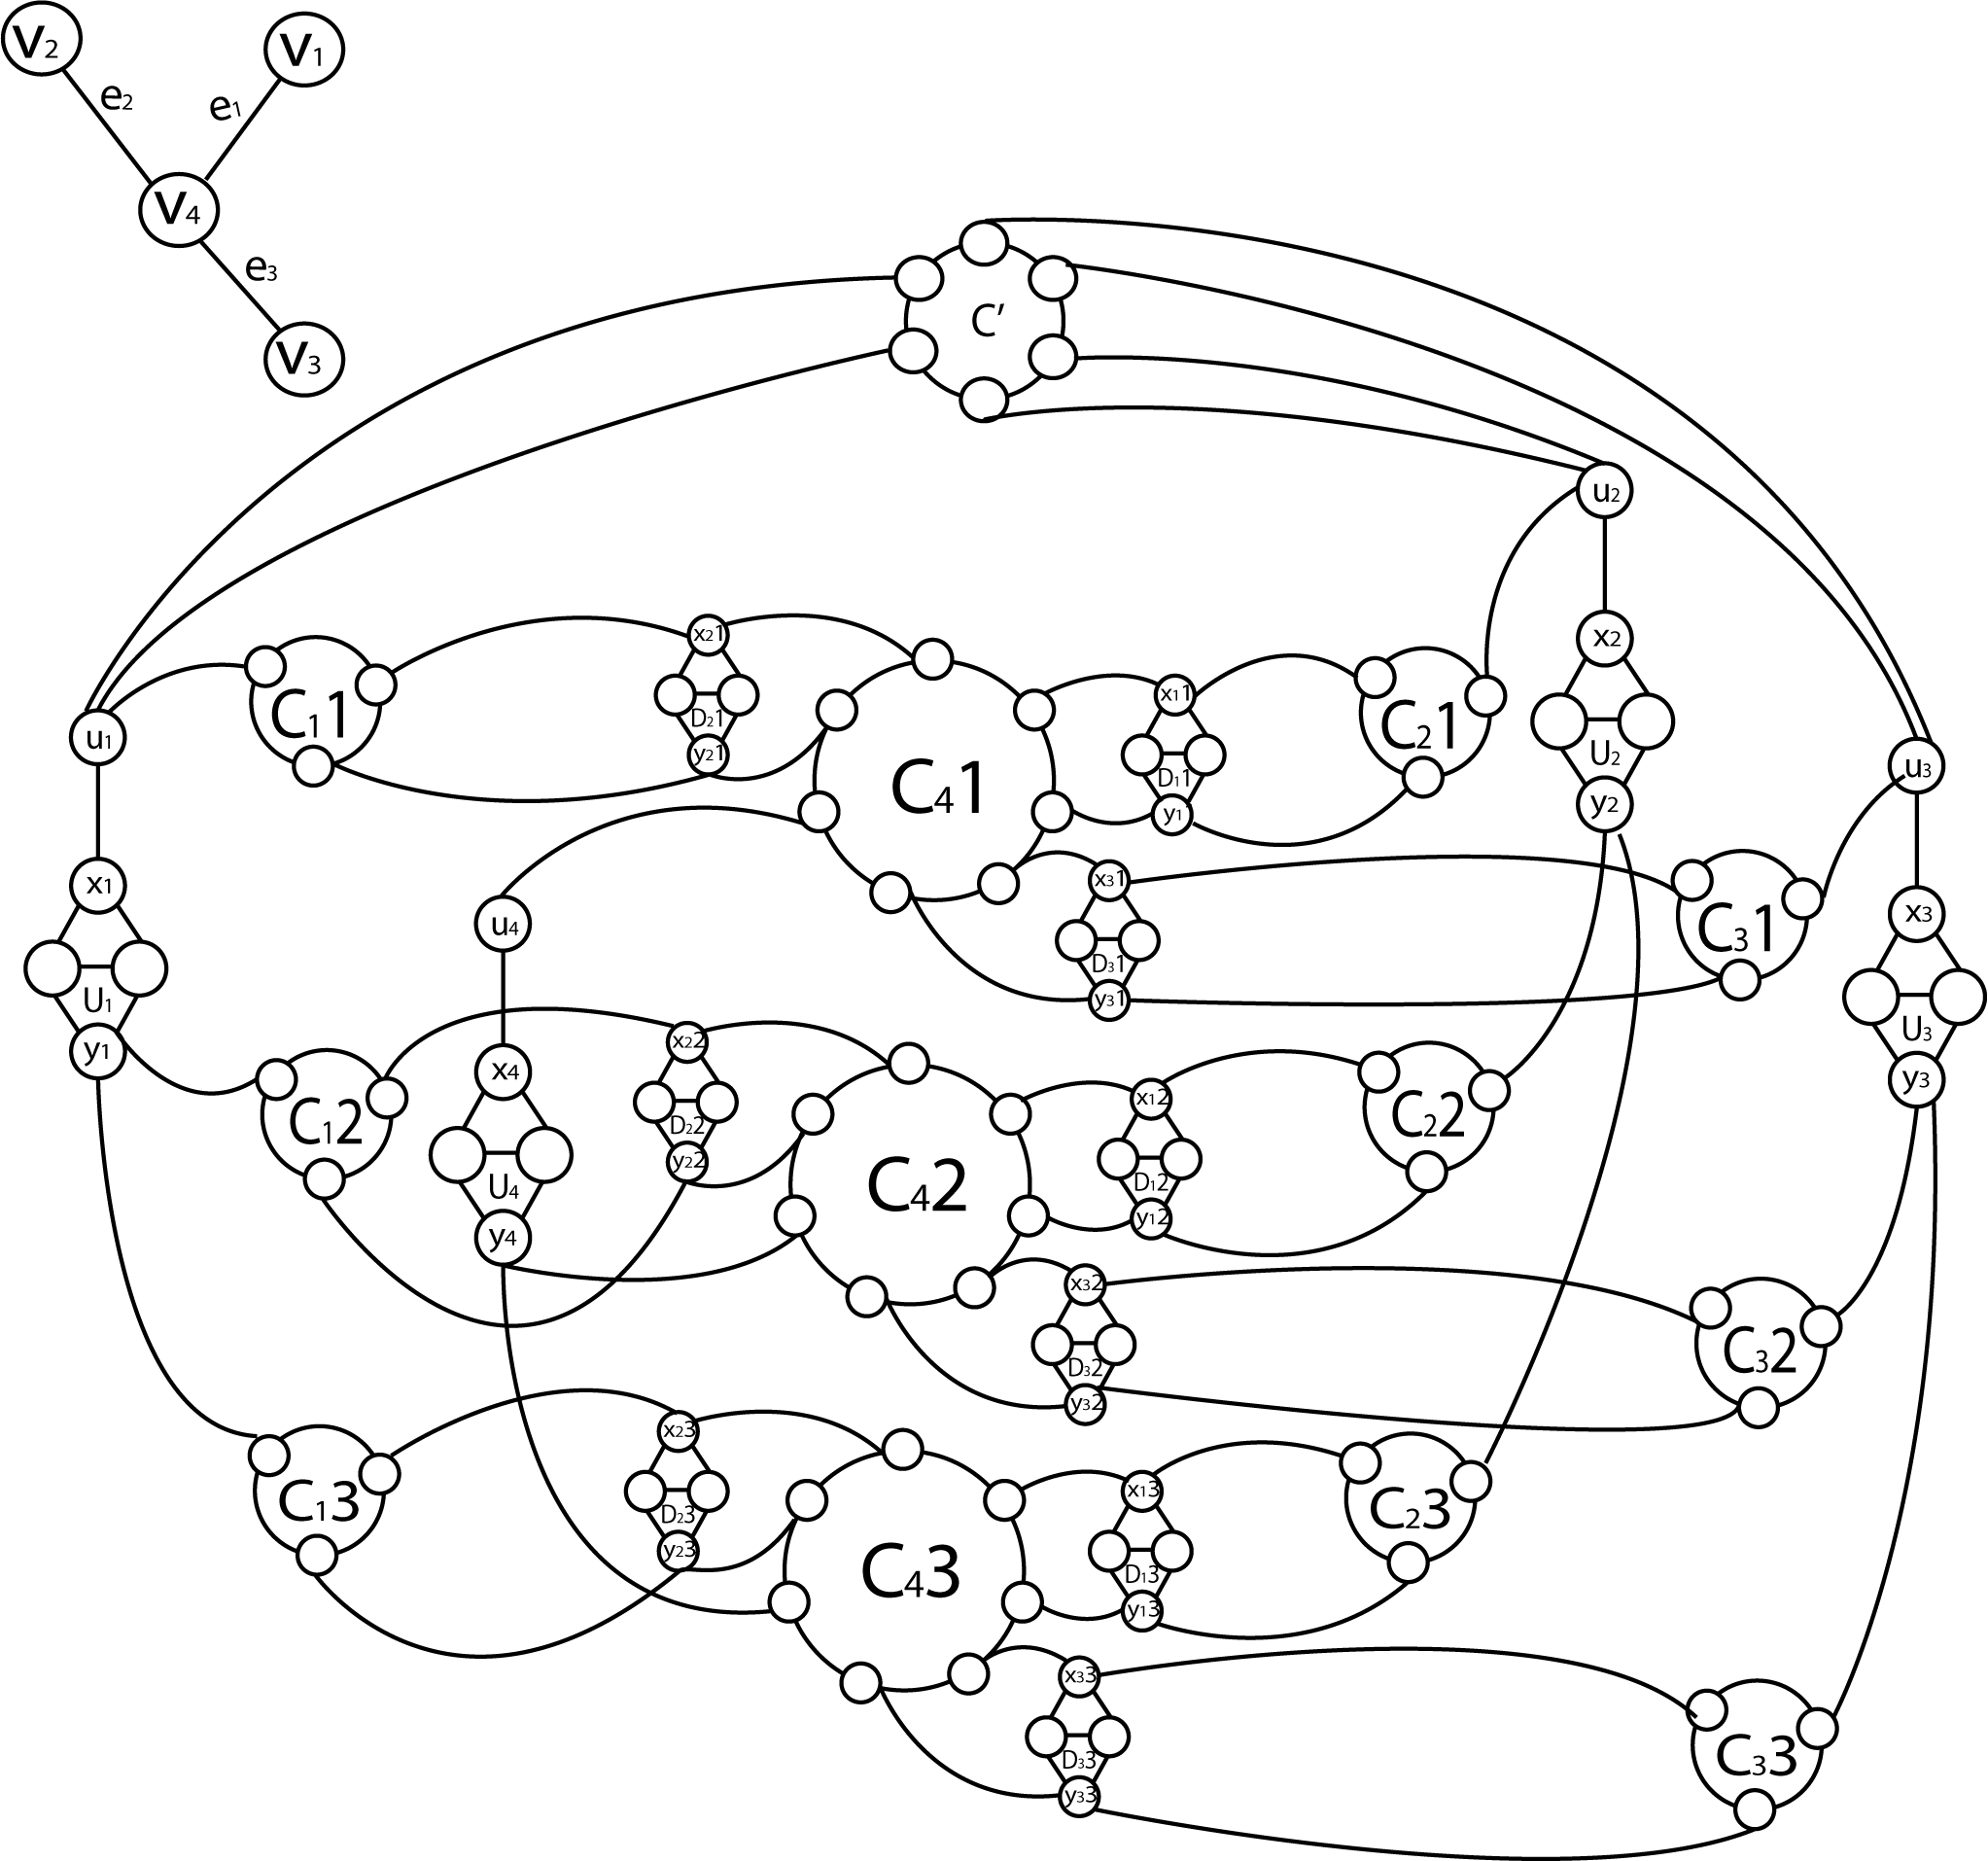
\includegraphics[width= 0.7\textwidth ]{img7.png}
\end{figure}
($\Rightarrow$) Sea $G$ un grafo $3$-coloreable, y una $3$-partici\'on de $V(G)$ tal que en cada conjunto $V_i$ queden solo v\'ertices de una mismo 
color de $G$, entonces existe un grafo $G'[H]$, subgrafo inducido de $G'$ que es $3$-regular, ya que siempre podemos tomar los v\'ertices de la siguiente forma:\\

\begin{enumerate}
    \item Todos los v\'ertices $a_{ij}$ est\'an en $H$
    \item Todos los v\'ertices $u_{i}$ est\'an en $H$
    \item Si $v_i$ de $G$ est\'a en el conjunto $V_c$ de la tricoloraci\'on, entonces los v\'ertices $c_{ij}$ del ciclo $C_i^c$ est\'an en $H$.
    \item Si $c ~\neq ~1$ para el conjunto $V_c$ al que pertenece $v_i$, entonces los v\'ertices de $U_i$ pertenecen a $H$.
    \item Si la arista $e_j$, es adyacente al v\'ertice $v_i$ que est\'a en el conjunto $V_c$, entonces los v\'ertices de $D_j^c$ adyacente a $C_i^c$ est\'an en $H$.
\end{enumerate}
    El subgrafo $G'[H]$ existe para cualquier $3$-partici\'on de $G$, y cuando la $3$-partici\'on corresponde con una 
    coloraci\'on se puede comprobar que todos los v\'ertices en $G'[H]$ tienen grado $3$, en principio en $G'$ todos los v\'ertices son de grado $3$ excepto los 
    $x_{jp}^c$ y $y_{jp}^c$ de los $D_{jp}^c$ que son de grado $4$ pero en el subgrafo se hace una construcci\'on a partir de una coloraci\'on y en $G'$ los $D_{jp}^c$ grafos reemplazad aristas, 
    entonces los v\'ertices $x_{jp}^c$ y $y_{jp}^c$ est\'an conectados a v\'ertices de c\'irculos que no pertenecer\'an ambos a $H$, de donde obligatoriamente quedan en grado $3$. De igual modo ocurre con los v\'ertices $u_i$ y $y_i$ de los $U_i$, quienes tienen 
    grado $4$ cada uno en $G$, pero como $H$ lo formamos considerando la $3$-partici\'on y cada v\'ertice puede estar s\'olo en uno de los $3$ conjuntos, entonces de las aristas que inciden en $u_i$ solo se quedan las $2$ que lo conectan al ciclo $C'$ y la que se corresponde a si $v_i$ 
    est\'a en el conjunto $V_1$ o no, y en los casos en los que se toma alg\'un $y_i$ como parte del conjunto $H$, en \'el solo permanecen las dos aristas que lo conectan al resto del $U_i$ y solo una de las que indica si el v\'ertice est\'a en el conjunto $V_2$ o en el $V_3$ de la $3$-partici\'on. 
    Por tanto en $G'[H]$, todos los v\'ertices tienen grado $3$.\\ 

($\Leftarrow$) Si $G'$ contiene un subgrafo $3$-regular $G'[H]$, entonces sobre $H$ se cumplen las siguientes propiedades:\\ 

\begin{enumerate}
    \item Todos los v\'ertices $a_{pi}$ y $u_i$ pertenecen a $H$.
    \item Por cada $i$, $1~ \leq~i~\leq ~n$, exactamente uno de los ciclos $C_i^{h}$ est\'a en $H$.
    \item Por cada $i$, $1~ \leq~i~\leq ~n$, si $C_i^{h}$ est\'a en $H$, entonces ning\'un otro $C_j^{h}$ para toda $j$ tal que $<i,j> \in E(G)$.
\end{enumerate}

\textbf{Dem 1.}: Supongamos que en $H$ no est\'a alguno de los $u_i$, como ese v\'ertice no estar\'ia sus adyacentes en $C'$ quedar\'ian con grado $2$ por lo que no podr\'ian estar en $H$, esto romper\'ia el ciclo $C'$ produciendo 
que ninguno de sus v\'ertices est\'e en $H$ y estos a su vez al no poder estar en $H$, reducir\'ian en $2$ la cantidad de aristas de los restantes $u_i$ por lo que ninguno de los $u_i$ podr\'ia estar en $H$. Como cada $u_i$ es adyacente a un v\'ertice de los $C_i^1$, no se pudiera tener ning\'un v\'ertice de los $C_i^1$ en $H$
y la eliminaci\'on de estos v\'ertices quita la posibilidad a los de $D_j^1$ de pertenecer a $H$. De igual modo cada $u_i$ es adyacente al $x_i$ de los $U_i$, de donde ning\'un v\'ertice de los $U_i$ podr\'ia estar en $H$ ya que $x_i$ pasar\'ia a tener grado $2$, al no poder estar, tampoco podr\'ian $u_{i1}$ y $u_{i2}$ quienes al quitar $x_i$ 
quedar\'ian con grado $2$ y como esos tampoco estar\'ian, se debe quitar tambi\'en $y_i$, este \'ultimo al estar conectado con un v\'ertice de $C_i^2$ y  con uno de $C_i^3$ hace que estos queden con grado $2$ por lo que rompen los ciclos 
haciendo que ninguno de sus v\'ertices puedan estar en $H$, esto finalmente provoca que los v\'ertices de $D_i^2$ y $D_i^3$ tampoco puedan estar en $H$, quedando $H = \emptyset$.\\ 

Por tanto todos los $u_i$ tienen que estar en $H$ y esto condiciona que todos los $a_{pi}$ est\'en en $H$ ya que, entre las $3$ aristas que permanezcan incidiendo en $u_i$ en el subgrafo c\'ubico 
una de ellas obligatoriamente est\'a conectada a uno de los $a_{pi}$, como los $a_{pi}$ todos tienen grado $3$ y son adyacentes a otros dos $a_{p'i'}$, si uno de ellos est\'a, todos tienen que estar.\\ 

\textbf{Dem 2.}: Como todos los $u_i$ est\'an en $H$ y los $a_{pi}$, entonces para que $u_i$ tenga grado $3$ en el grafo inducido por $H$, es necesario que a $H$ se agregue o bien el v\'ertice de $C_i^1$ al que $u_i$ es adyacente o el 
$x_i$, pero nunca ambos. En caso que se agregue el v\'ertice adyacente en $C_i^1$, entonces todo el ciclo se debe agregar ya que el grado $3$ de cada uno de los v\'ertices depende de los restantes. En caso que se agregara el $y_i$ este para completar su grado $3$
requiere que se agregue el resto de los v\'ertices del $U_i$ y que para completar el grado $3$ de $y_i$ se agregue o bien su adyacente en $C_i^2$ o  en $C_i^3$, pero nunca ambos porque si no, pasar\'ia a tener grado $4$. Con la adici\'on de uno de estos v\'ertices a 
$H$ se debe agregar todo el ciclo $C_i^h$ al que pertenece por los mismos motivos que se agregar\'ia $C_i^1$ en el caso anterior. De este modo se garantiza que para cada $i$, se agrega uno y solo uno de sus $C_i^h$ ciclos.\\ 

\textbf{Dem 3.}: 

Si a $H$ pertenecen los v\'ertices de $C_i^h$, como todos ellos tienen degree exactamente $3$, todos sus vecinos tienen que pertenecer tambi\'en a $H$, de donde 
los v\'ertices de los $D_j^h$ de las aristas $e_j$ que inciden en $v_i$ en $G$ pertenecen a $H$ y los 
v\'ertices $x_j^h$ y $y_j^h$ est\'an conectados a v\'ertices de $C_i^h$ y tienen que para alcanzar el grado $3$ obligatoriamente incluir a todos los v\'ertices de  
$D_j^h$; por lo que si para alg\'un $v_k$ adyacente a $v_i$, el ciclo $C_k^h$ tambi\'en estuviese en $H$, sea $e_{j'}$ la arista que une a $v_i$ con $v_k$, los v\'ertices $x_{j'}^h$ y $y_{j'}^h$  tienen que 
tener tanto la arista que los conecta con uno de los v\'ertices de $C_i^h$ como la que los conecta con uno de los v\'ertices de $C_k^h$, adem\'as de que obligatoriamente tienen que estar conectados a sus dos adyacentes en $D_{j'}^h$ porque 
al menos tienen que incluir uno y esto condiciona que se agregue el otro al ser adyacentes entre ellos y tener grado exactamente $3$, por lo que en ese caso  $x_{j'}^h$ y $y_{j'}^h$ quedar\'ian con degree $4$, por tanto si $C_{i}^h$ est\'a en $H$, ning\'un 
 $C_k^h$ tal que $v_k$ adyacente a $v_i$ en $G$, puede estar en $H$. \\
 

Por la proposici\'on (2) implica que el subgrafo $G'[H]$ es una $3$-partici\'on de los v\'ertices de $G'$ tal que el v\'ertice
$v_i$ est\'a en la partici\'on $c$ si $C_i^c \in H$. La proposici\'on (3) asegura que v\'ertices adyacentes est\'en en diferentes conjuntos en la partici\'on, de donde
si $G'$ tiene $G'[H]$ como subgrafo c\'ubico, entonces $G$ es $3$-coloreable. $\Box$  \\ 

\subsection*{Reducci\'on implementada}
Con el objetivo de probar en la pr\'actica la reducci\'on del problema $3$-coloreable al problema del subgrafo c\'ubico, se program\'o la trasformaci\'on de 
la entrada de un problema al otro en la funci\'on \texttt{Reduction} del archivo \texttt{Reduction.py}. Adem\'as se programaron las soluciones backtrack para ambos problemas,
de modo que se pueda comprobar que cuando el algoritmo backtrack para determinar si un grafo es $3$-coloreable devuelva \textit{True} para alguna entrada, entonces el algoritmo 
de backtrack para subgrafo $3$-regular también ha de devolver \textit{True} para el grafo obtenido de la reducc\'ion, an\'alogamente para los casos en que el resultado sea \textit{False}.\\ 

La funci\'on \textit{Reduction} realiza las siguientes operaciones: 

\begin{itemize}
    \item[$\circlearrowright $] Crea e inicializa la matriz de adyacencia de G: $n^2 + m$
    \item[$\circlearrowright $] Determina los degrees de cada v\'ertice: $n^2$
    \item[$\circlearrowright $] Realiza el paso (1) de la reducci\'on: $n * 3(2n-1)$
    \item[$\circlearrowright $] Crea las $K'_4$ del paso (2): $m$
    \item[$\circlearrowright $] Conecta las $K'_4$ creados al grafo: $m * 4(2n-1)$
    \item[$\circlearrowright $] Crea los $K'_4$ m\'as un v\'ertice del paso (3) y los conecta: $n(2n -1) $
    \item[$\circlearrowright $] Crea el ciclo $C'$ del paso (4) y lo conecta al grafo: $2n$
    \item[$\circlearrowright $] El grafo creado tiene un m\'aximo de $6n^2 + 4n + 12m$ v\'ertices
    \item[$\circlearrowright $] Crea la matriz de adyacencia para el nuevo grafo y las aristas: $2(6n^2 + 4n + 12m)^2$
\end{itemize}

Por lo que el costo de la reducci\'on cumple:

$$T(n,m) \leq 2n^2 + 2m + 4n(2n-1) + 4m(2n-1) + 2n + 2(6n^2 + 4n + 12m)^2$$
$$\leq 2n^2 + 2m + 4(2n-1)(n+m) + 2n + 2(6n^2 + 4n + 12m)^2$$

Como $m \leq \frac{n(n-1)}{2} \leq n^2$ entonces

$$T(n,m) \leq 4n^2 + 4(2n-1)(n+n^2) + 2n + 2(18n^2 + 4n)^2 \leq Kn^4$$ 

donde $K$ es una constante lo suficientemente grande, de donde $T(n,m) = O(n^4)$, por lo 
que se pude computar la reducci\'on en tiempo polinomial.

\subsection*{Soluci\'on Backtrack para el problema del subgrafo c\'ubico}
La soluci\'on exacta al problema del subgrafo $3$-regular fue programada haciendo uso de un algoritmo de Backtrack en el que para cada una de las aristas del grafo se tienen 
dos posibles opciones, esta forma parte del subgrafo $3$-regular o no, por tanto se genera un \'arbol binario en el que cada rama corresponde a la eliminaci\'on o no de una arista
del grafo, para ser parte del subgrafo. Luego de que se haya pasado por todas las aristas decidiendo si ponerlas o no, en el caso base se comprueba que el grado de todos los v\'ertices sea $3$ o $0$
y que adem\'as no todos sean $0$. Esta primera variante (top-down) genera todos los posibles subgrafos de $G$, por lo que tiene $2^m$ posibles subgrafos finales a analizar, el c\'odigo de la misma se encuentra
en la funci\'on \texttt{BacktrackCubicSubgraph} del archivo \texttt{BacktrackCubicSubgraph.py}.\\ 

Para mejorar el costo del Backtrack, fue implementada una soluci\'on bottom-up, en la que inicialmente se asume el grafo $G$ sin aristas y 
se va decidiendo por cada arista la opci\'on de agregarla o no al grafo, comprobando que se pueda agregar antes de hacerlo, en caso contrario se poda esa rama 
del \'arbol de recursividad. De igual modo en el caso base comprueba que no todos los v\'ertices hayan quedado con grado $0$ y que todos tengan grado $0$ o $3$. 
Esta implementaci\'on se encuentra en el m\'etodo \texttt{BacktrackCubicSubgraph}, tanbi\'en en el archivo \texttt{BacktrackCubicSubgraph.py}.

\subsection*{Soluci\'on Backtrack para el problema del grafo 3-coloreable}

Para determinar si un grafo es $3$-coloreable tambi\'en se programaron dos algoritmos de backtrack, el primero computa todas las posibles 
combinaciones de colores que se le pueden dar a los $n$ v\'ertices del grafo y una vez que tiene una nueva combinaci\'on se eval\'ua que para cada 
``color'' se tenga que los v\'ertices que est\'an en ese conjunto formen un conjunto independiente, en caso afirmativo el grafo es $3$-coloreable, y si no se procede a formar 
otra posible combinaci\'on. La cantidad de combinaciones posibles equivale a la forma de repartir $n$ objetos iguales en $3$ categor\'ias diferentes, es decir $n^3$ posibles caos.\\ 

Para podar el backtrack se implement\'o otro algoritmo que antes de asignarle un color a un v\'ertice comprueba que no tenga vecinos en dicho grupo. De este modo se pueden 
eliminar asignaciones que sabemos no van a ser efectivas. Estos algoritmos se encuentran programados en las funciones \texttt{ThreeColorableBacktrack} y \texttt{ThreeColorableB} respectivamente, ambos en el archivo 
\texttt{Backtrack3Coloreable.py}.

\subsection*{Generador de casos pruebas}

Para generar casos de prueba generamos grafos con un total de v\'ertices aleatorio $n \in [4;100], n \in \mathbb{N}$ (la cota m\'inima fue $4$ producto que para menos que eso es trivial que el grafo es $3$-coloreable) 
de igual modo se seleccion\'o una cantidad $m$ aleatoria de aristas con $m \in [n-1; \frac{n(n-1)}{2}]$, las cuales se agregaron entre v\'ertices aleatorios. Se busc\'o que el grafo fuera conexo haciendo un recorrido BFS, si un nodo no fue alcanzado 
se conect\'o con alguno de los v\'ertices de esa componente aleatoriamente. Se repite este proceso hasta que todos est\'an conectados. La decisi\'on de conectar el grafo se debe a que, el subgrafo $3$-regular tienen respuesta afirmativa 
si y solo si para alguna componente conexa existe el subgrafo, mientras que grafo $3$-coloreable tiene respuesta afirmativa si y solo si todas sus componentes conexas se pueden pintar con $3$ colores.\\ 







\subsection*{Cuestiones sobre subgrafos 3-regulares}

\textbf{Teorema}: Para todo $p$ primo, cualquier grafo $G=(V,E)$ tal que el promedio de los grados de sus v\'ertices sea mayor que 
$2p-2$ y el $\Delta(G)$ sea a lo sumo $2p -1$, tiene un subgrafo $p$-regular.\\ 

\textbf{Demostraci\'on}: Sean los valores binarios $a_{i,j}$, tales que $a_{i,j} = 1$ si la arista $e_{j}$ incide en el v\'ertice $v_i$, $a_{i,j} = 0$ en otro caso.
Considerando el polinomio de variables $x_e,~ e\in E(G)$:

$$P(x_e) = \prod_{v \in V(G)} \left( 1 - \left(\sum_{e \in E(G)} a_{ve} x_e\right)^{(p-1)}\right) - \prod_{e \in E(G)} (1 - x_e)$$ 

Como se tiene que el grado promedio es mayor que $2p-2$, entonces: 

$$\frac{2|E|}{|V|} > 2p-2 $$
$$|E| > (p-1)|V|$$

Por tanto, se tiene que el grado de $P$ es $|E| = \sum_{e \in E} t_e$, donde $t_e = 1$ para $e \in E$, luego se tiene que el 
coeficiente principal del polinomio es $- \prod_{e \in E}  - x_e^{t_e} = - \prod_{e \in E} - x_e = (-1)^{|E| + 1} \neq 0$. Sean los 
conjuntos de soluci\'on $S_e = {0,1}$ para toda $e \in E$, como $|S_e| > t_e$ para toda $e \in E$, entonces por el Corolario del \textit{Teorema Combinatoria Nullstellensatz}, se tiene 
que existe $s_e \in S_e$, tales que $P((s_1,...s_m))  \neq 0$. Dicho vector no es el vector $0$, ya que $P(0) = \prod_{v \in V(G)}  1 - \prod_{e \in E(G)} 1 = 1 - 1 = 0$. De aquí se tiene que entonces 
como alg\'un $s_e$ debe ser igual a $1$, entonces $\prod_{e \in E(G)} (1 - s_e) = 0$, de donde para cada $v \in V$ se tiene que cumplir que 
$\sum_{e \in E(G)} a_{ve} x_e \equiv 0$ (mod $p$), puesto que de lo contrario por el \textit{Peque\~no Teorema de Fermat} se tiene que $(\sum_{e \in E(G)} a_{ve} s_e)^(p-1) \equiv 1$ (mod $p$), de donde 
$P((s_1,...,s_m)) = 0 $. Por tanto en el subgrafo conformado por las aristas $e$ tales que $s_e = 1$, se tiene que todos los v\'ertices extremos de estas aristas tendr\'ian grado $p$, puesto a que para ellos
$(\sum_{e \in E(G)} a_{ve} s_e) > 0$, divisible entre $p$ y menor que $2p-1$. $\Box $


\subsection*{Algoritmo gen\'etico para determinar la existencia de subgrafo c\'ubico}

Una alternativa para dar con la existencia o no de un subgrafo cúbico es utilizar técnicas de Inteligencia Artificial. En esta sección propondremos un algoritmo genético para decidir si un grafo cualquiera tiene un subgrafo cúbico. Para recordar un poco un algoritmo genético suele contar con una población solución inicial; una función fitness para evaluar cada solución, la cual se quiere minimizar o maximizar; un función de selección de la población; una operación de cruce de soluciones; posibles funciones de mutaciones, y de nueva generación de soluciones. La propuesta fue la siguiente:

\begin{itemize}
	\item Función de generación individual: Genera aleatoriamente un subgrafo del grafo original.
	\item Función de selección con torneo: En cada etapa, se hace una mezcla de la población y se agrupan en parejas, varias soluciones, las cuales se evalúan con la función de fitness y la ganadora pasa a formar parte de la selección
	\item Función de cruce de punto fijo: Se hace una bipartición de los nodos del grafo original, y se crean 2 soluciones nuevas que llamaremos, hijo 1 e hijo 2, utilizando 2 soluciones previamente que llamaremos padre 1 y padre 2. El hijo 1 adquiere todas las aristas que tenga el padre 1 entre los nodos de uno de los conjuntos de la bipartición, y también adquiere todas las aristas de que tenga el padre 2 entre los nodos del otro conjunto de la bipartición. Análogamente el hijo 2 adquiere las aristas de esta manera pero del padre 2 primero, y luego del padre 1. Note que las aristas que existían entre los 2 conjuntos de los nodos, no son heredadas por ninguno de los hijos.
	\item Funciones de mutación:
	\begin{itemize}
		\item Mutación 1: Agregar una arista válida al grafo. Arista válida se traduce a una arista que está en el grafo original
		\item Mutación 2: Quitar una arista del grafo
		\item Mutación 3: Agregar todas las aristas válidas de un vértice.
		\item Mutación 4: Quitar todas las aristas de un vértice, es decir, aislar el vértice. 
	\end{itemize}
	\item Función de fitness:
	\begin{itemize}
		\item Fitness 1: Para cada uno de los vértices se calcula el grado de cada vértice, y se suman las mínimas de las distancias entre el grado de cada uno, y $0$ o $3$. Note que si un grado tiene grado $1$, al estar más cerca de $0$ sumaría al fitness total $1$. y del mismo modo sucede si el vértice tuviera grado $2$, este estaría más cerca de $3$ y aportaría $1$ al fitness. En cambio un nodo con grado $9$ está más cerca de $3$, y tiene una distancia de $6$, la cual influiría en el valor del fitness. Note que el fitness sería $0$, solo cuando los grados de los nodos son $0$ o $3$ (no necesariamente todos a la vez), sin embargo para nuestro problema no es válido que todos los nodos sean de grado, $0$, por lo tanto en dicho caso, se penaliza el fitness con la la mitad de la sumatoria de los grados de los vértices del grafo original.
		\item Fitness 2: Se fija un valor $p$ que representará un grado pivote. Mientras más alejado de $p$ esté el grado de un vértice, más penalización recibirá el fitness. Sin embargo la penalización es más fuerte para los grados menores que $p$, ya que esta será:
		$$(p-x)*3)$$
		mientras que para los grados mayores o iguales que $p$, la penalización será menos brusca:
		$$\frac{(x - p + 3)}{3}$$
		Sin embargo, si el grado del vértice es $0$ o $3$, el vértice no afectará al fitness, a no ser que todos los nodos tengan grado $0$ en ese caso, recibirá una penalización igual a lo explicado en la función 1. Note que esta función es $0$ solo cuando el grafo armado tiene un subgrafo 3-regular.
	\end{itemize}	
\end{itemize}

El algoritmo genético implementado, consiste en generar una población de 200 soluciones con la función de creación individual. Luego hacer una selección del $75\%$ de la población mediante la función de selección con torneo. Crear una cantidad igual de hijos a la población seleccionada, producto del cruce con punto fijo. Luego realizar mutaciones a algunos hijos. Y finalmente rellenar con soluciones aleatorias nuevas, hasta tener nuevamente una población de 200 soluciones. Este proceso se repite varias veces, hasta que una solución obtiene fitness $0$, o hasta que hayan sucedido cierto número de operaciones.

Las experimentaciones que hicimos arrojaron mejores resultados al seleccionar la segunda función de fitness y solamente las mutaciones de eliminación y agregado de aristas. Lo primero tiene más sentido, ya que una solución cuyos grados de los nodos están más cercanos del $0$ o del $3$ no suele resolverse tan fácil quitando o poniendo pocas aristas, sino que por lo general esta solución estaría mucho más apartada de alguna solución real, haciendo cambios de este estilo. Por lo tanto la segunda función de fitness nos garantiza que se explore más por otras vías, y la búsqueda no quede tan sesgada.

Ahora bien, algo más que se añadió a la función de fitness para reconocer si el grafo tenía un subgrafo cúbico, fue utilizar el Teorema explicado en la sección anterior. Note que al ser $3$ un número primo el teorema nos garantiza que un grafo contiene un subgrafo cúbico si el promedio de los grados de sus vértices es mayor estricto que 4, y el grado máximo es 5. Entonces si a la función de fitness le agregamos que cuando esta condición ocurra, dé como valor $0$, entonces nuestro algoritmo genético tendrá más opciones para hallar la solución.

Para comprobar la efectividad de este algoritmo se hicieron varias pruebas sobre varios grafos que se sabían que tenían subgrafos cúbicos, y sobre otros que se desconocía. Los subgrafos que sí se conocía que tenían subgrafos cúbicos se generaron con el modulo networkx de Python, el cual permite generar aleatoriamente grafos 3-regulares. A estos grafos solamente tuvimos que añadirle aleatoriamente más vértices. Se generaron más de 30 grafos, por cada cantidad de nodos fijados. Como las computadoras en las que corrimos estos casos de pruebas no son muy modernas utilizamos valores entre 10 y 40 nodos. Por cada caso de prueba ejecutado se aplicó el algoritmo genético 3 veces, para también contabilizar cuántas veces se fallaban adicionalmente, y como seguridad, por si la población inicial creada era muy mala. A continuación mostramos alguno de los gráficos de convergencia para los casos en donde el grafo sí contenía un subgrafo 3-regular:

\begin{figure}
	\centering
	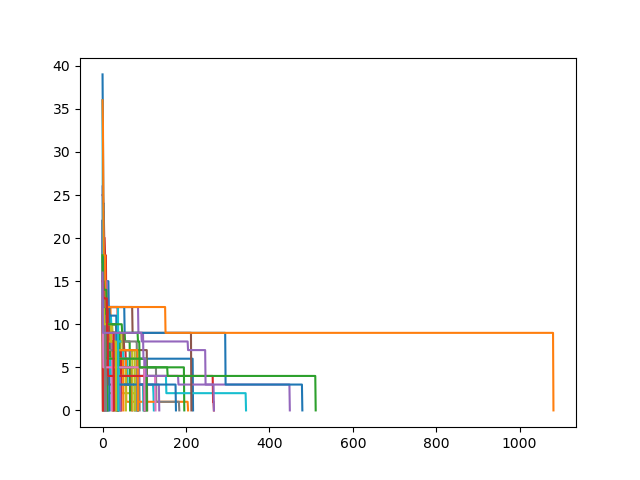
\includegraphics[width=0.7\linewidth]{converge_14.png}
	\caption{Convergencia en grafos de 14 nodos que contenían subgrafos cúbicos}
\end{figure}


Para los casos de pruebas con grafos de 14 nodos, la tasa de falsos positivos fue de $0.125$, y para los casos positivos el promedio de convergencia estuvo en $98.21$ iteraciones, con una desviación estándar de $155.35$. Este análisis para lo que nos sirve es para tener una idea de qué cota poner al número de iteraciones para decantarnos por el hecho de que no tenga subgrafo cúbico. Es importante aclarar que los falsos negativos se reconocieron que eran falsos usando el algoritmo de backtrack.

\subsection*{Algoritmo gen\'etico para determinar si el grafo es 3-coloreable}

Por otra parte la alternativa con Inteligencia Artificial para verificar si un grafo es 3-coloreable o no, fue aplicar nuevamente otro algoritmo genético. En este caso las soluciones serían una partición en 3 conjuntos, los cuales serían los colores con los que se colorea cada nodo.

\begin{itemize}
	\item Función de generación individual: Genera aleatoriamente una partición de los nodos en 3 conjuntos.
	\item Función de selección con torneo: En cada etapa, se hace una mezcla de la población y se agrupan en parejas, varias soluciones, las cuales se evalúan con la función de fitness y la ganadora pasa a formar parte de la selección
	\item Función de cruce de punto fijo: Se hace una bipartición de las dos soluciones padres. El hijo 1, tomaría la misma coloración del padre 1 según el primer conjunto de la bipartición, y heredaría la misma coloración del padre 2 según el segundo conjunto de la bipartición. Para el hijo 2 el proceso es análogo pero primero tomando al padre 2 y luego al padre 1.
	\item Función de mutación: Se cambia un color aleatorio de la solución.
	\item Función de fitness: Se contabilizan las incompatibilidad de color entre 2 nodos. Esto quiere decir que por cada par de nodos adyacentes con el mismo color, el fitness se incrementa en 1. Note que el fitness es 0 cuando el grafo es 3-coloreable.
\end{itemize}

El algoritmo genético en este caso es muy parecido al explicado anteriormente, solo diferenciándose en que la selección se hace 2 veces, con toda la población y se cruzan generando una cantidad de hijos igual que el tamaño de la población. Luego varios de los hijos son sometidos a mutación y se pasa a la siguiente etapa.

Aunque tenemos forma de saber cuán efectivo es el algoritmo genético del subgrafo cúbico, otra forma de comprobar la efectividad del mismo es comparar los valores de los resultados del algoritmo genético que reconoce 3-coloreables, con el algoritmo genético del subgrafo cúbico evaluado en el mismo grafo pero con la transformación de equivalencia entre estos 2 problemas NP. Este código se encuentra anexado (archivo Transform.py), pero aclaremos que la transformación genera grafos bastante grandes, como por ejemplo el que se encuentra en el notebook de Jupyter, donde un grafo de 4 vértices se transformó en un nuevo grafo de 184 vértices. Evaluar esto en los equipos que disponemos es en vano para muchos grafos, por lo tanto, se deja al lector esta comprobación. No obstante, tenga en cuenta en la sección anterior la vía con la cual se verificaba la efectividad del algoritmo genético de subgrafos cúbicos.

	

\subsection*{Complicando el problema, como si ya no estuviera complicado}
Aunque el problema de determinar si un grafo tiene un subgrafo c\'ubico es un problema puramente de decisi\'on, 
si se modifica un poco la orientaci\'on del problema se puede buscar escribir problemas que sean de optimizaci\'on 
aunque ello implique que se pierda la rigurosidad de que el grafo tenga realmente un subgrafo $3$-regular o que 
sea necesario agregar nuevas restricciones.\\


Una primera idea es la de maximizar la cantidad de v\'ertices del grafo que quedan con degree $0$ o $3$ luego de haber 
removido un conjunto de aristas del grafo, sin quitarlas todas, pero este problema tiene una soluci\'on aproximada mediante un greedy 
que es bastante buena, puesto que si la \'unica restricci\'on es no quitar todas las aristas, basta con dejar solo una 
y tendr\'iamos todos los restantes v\'ertices con degree $0$ excepto por los $2$ que quedar\'ian con degree $1$. N\'otese que el 
\'optimo de este problema en el mejor de los casos es $n$, que se alcanzar\'ia en el caso que el grafo tenga un subgrafo c\'ubico, mientras 
que con el greedy se tiene que el \'optimo es $n-2$ v\'ertices con degree $0$ o  $3$, por lo que la soluci\'on golosa solo se aleja en el peor caso 
en $2$ de la \'optima, siendo una buena aproximaci\'on.\\ 

Otra idea, restringiendo m\'as el problema es, no solo forzar a que tengamos al menos $1$ arista que no quitemos del grafo, sino 
a que al menos nos quede un v\'ertice de grado $3$, esto implica que en el grafo de entrada al menos tiene que existir un v\'ertice con grado 
mayor o igual a $3$. Por tanto tambi\'en se puede de forma greedy encontrar un valor cercano al \'optimo, si tomamos uno de los v\'ertices de grado mayor  
o igual que $3$ en el grafo y nos quedamos con $3$ de sus aristas, con lo que cumplimos la restricci\'on de tener al menos un v\'ertice de grado $3$ y en total 
quedar\'ian $n-3$ v\'ertices que cumplen la condici\'on de tener grado $3$ o $0$, lo cual dista en el peor caso en $3$ al resultado \'optimo que puede llegar a ser $n$
si tuvi\'eramos en el grafo un subgrafo $3$-regular.\\ 

Una tercera idea, esta s\'i enfocada en la detecci\'on de subgrafos $3$-regulares, es dado un grafo del que sabemos tiene al menos un subgrafo $3$-regular, determinar la cardinalidad del 
mayor subgrafo $3$-regular que tiene. Si para esta idea existiera un algoritmo polinomial que fuera un $\rho$-aproximaci\'on del \'optimo del problema, es decir que nos devolviese un valor $M'$
que $M'\rho \geq M$, es decir fuera, en el peor caso, $\rho$ veces menor que el resultado real del tama\~no m\'aximo del subgrafo $3$-regular, entonces ocurrir\'ia lo siguiente: \\ 


Sea $G$ un grafo del que se quiere determinar si es $3$-coloreable, tal que $|V(G)| >  \left\lceil\frac{2\rho}{5} \right\rceil $ y $G$ es conexo, si a partir de $G$, construimos un $G'$ utilizando la 
reducci\'on inicial, para obtener la entrada al problema de subgrafo c\'ubico, entonces sobre $G'$ sabemos lo siguiente: 

\begin{itemize}
    \item[$\triangle $] $G'$ tiene un subgrafo c\'ubico $\Leftrightarrow $ $G$ es $3$-coloreable.
    \item[$\triangle $] Si en $G'$ hay un subgrafo c\'ubico $G'[H]$ entonces: 
    \begin{itemize}
        \item[$\blacktriangle $] $C'$ est\'a en $H$, lo que aporta $2|V(G)|$ v\'ertices.
        \item[$\blacktriangle $] Por cada $v$ de $G$ hay un $C_i^h$ en $H$, lo que aporta $\sum_{v \in V(G)} 2*d(v) + 1 \geq 3|V(G)|$ v\'ertices.
        \item[$\blacktriangle $] Todos los $u_i$ est\'an en $H$, aportando $|V(G)|$ v\'ertices.
        \item[$\blacktriangle $] Por cada arista de $G$, en $H$ est\'an los $4$ v\'ertices de un $D_j^h$, como $G$ conexo entonces $4|E(G)| \geq 4(|V(G)| - 1) = 4|V(G)|-4$.
        \item[$\blacktriangle $] Como $|V(G)| > \left\lceil \frac{2 \rho}{5} \right\rceil \geq 1 $, entonces en $H$ alguno de los $C_i^h$ tiene $h =2,3$, por lo que en $H$ est\'an al menos los $4$ v\'ertices de alg\'un $D_i$.
        \item[$\blacktriangle $] $\therefore~ |H| \geq 2|V(G)| + 3|V(G)| + |V(G)| + 4|V(G)|-4 +4 = 10|V(G)|$
    \end{itemize}
\end{itemize}
Si a $G'$ le agregamos un $K_4$ m\'as un v\'ertice($x$), conectando este v\'ertice a uno de los v\'ertices de $C'$, de este modo obtenemos un $C''$ que siempre tiene alg\'un subgrafo c\'ubico y que por tanto 
servir\'ia de entrada para el algoritmo de $\rho$-aproximaci\'on. \\

N\'otese que si $G$ no es $3$-coloreable, entonces el mayor subgrafo $3$-regular de $G''$ es el $K_4$ que agregamos puesto a que $G'$ no tiene 
subgrafos $3$-regulares en este caso y al conectar el $K_4$ a $G'$ mediante el v\'ertice $x$ que tambi\'en agregamos, se garantiza que en el grafo $G''$ el $K_4$
agregado no expanda el tama\~no de ning\'un posible subgrafo ni genere otro nuevo distinto de \'el.\\ 

En cambio, si $G$ es $3$-coloreable el m\'aximo subgrafo c\'ubico de $G''$ tiene cardinalidad mayor o igual a $10|V(G)| + 4$, de donde si al utilizar el algoritmo de la $\rho$-aproximaci\'on 
este nos devolviese algo mayor que $4$ tendr\'iamos la certeza de que $G$ es $3$-coloreable porque el \'unico modo en que el subgrafo c\'ubico m\'aximo de $G''$ tenga m\'as de $4$ v\'ertices es en este caso. Tambi\'en si 
la respuesta del algoritmo fuese exactamente $4$ (No puede ser menor porque no hay grafo c\'ubico de menos de $4$ v\'ertices) podemos asegurar que $G$ no es $3$-coloreable, ya que la $\rho$-aproximaci\'on en el peor caso devuelve un m\'aximo que es $\rho$ veces 
peor que el real, de donde se tendr\'ia 

$$M'\rho \geq M \Rightarrow 4\rho \geq M$$

Como $M \geq 10|V(G)| + 4$, entonces: 

$$4\rho \geq 10|V(G)| + 4 > 10|V(G)| \Rightarrow \frac{4\rho}{10} \geq |V(G)| \Rightarrow \frac{2\rho}{5} \geq |V(G)|$$

Pero como sabemos que $|V(G)| >  \left\lceil\frac{2\rho}{5} \right\rceil $, entonces jam\'as ser\'ia devuelto $4$ por el algoritmo en caso que hubiese un subgrafo $3$-regular mayor.\\ 

Adem\'as para todo grafo $G_0$, con cantidad de v\'ertices $n$ existe un grafo $G$ con cantidad de v\'ertices $|V(G)| >  \left\lceil\frac{2\rho}{5} \right\rceil $, tal que $G_0$ es $3$-coloreable $\Leftrightarrow$ $G$ es $3$-coloreable. Esto se consigue de la 
siguiente forma, sea $k = \left\lceil\frac{2\rho}{5} \right\rceil - n$, si $k < 0$ ya $G_0$ tiene la cantidad de v\'ertices necesarios, en caso contrario creamos un grafo $P_{k+1}$ y conectamos uno de sus extremos a cualquier v\'ertice de $G_0$, si $G_0$ no era $3$-coloreable 
agregarle v\'ertices en ninguna circunstancia reduce el n\'umero de colores con los que se puede pintar un grafo. Mientras que, si $G_0$ fuese $3$-coloreable, como $P_{k+1}$ se puede colorear con $2$ colores, dada una tripartici\'on de $G_0$ que se corresponda con una coloraci\'on, basta con determinar en 
cuál de los $3$ conjuntos est\'a el v\'ertice al que uniremos con el $P_{k+1}$ y luego colorear correctamente los v\'ertices del $P_{k+1}$ con los $2$ colores que no contienen a dicho v\'ertice.\\ 

De modo que si para el problema planteado hubiera una $\rho$-aproximaci\'on, el problema de determinar cuando un grafo es $3$-coloreable se resolver\'ia en tiempo polinomial, por tanto dicho algoritmo de $\rho$-aproximaci\'on no 
puede existir. $\Box $.

\end{document}